\documentclass{beamer}
%Information to be included in the title page:
% \title{Sample title}
% \author{Anonymous}
% \institute{Overleaf}
\usepackage{booktabs}
\usepackage{graphicx}
\usepackage{subcaption}
\usepackage[]{hyperref}

\usetheme[]{default}
\begin{document}
\renewcommand{\d}{\: \mathrm{d} }
\newcommand{\e}{\mathrm{e}}


\title[] {Recitation Class 3}

\author[lzx]{Zexi Li}

\institute[email]{lzx12138@sjtu.edu.cn}

\date{2021.06.01}

\frame{\titlepage}

\AtBeginSection[]
{
  \begin{frame}
    \frametitle{Table of Contents}
    \tableofcontents[currentsection]
  \end{frame}
}

\begin{frame}
    \frametitle{Outline}
    \tableofcontents
\end{frame}


\section{Chapter 4-II The Semiconductor in Equilibrium}
    \begin{frame} \frametitle{One More Equation}
        \begin{equation*}
            \boxed{E_{Fi} - E_{midgap} = \frac{1}{2} kT \ln \left( \frac{N_v}{N_c}  \right) = \frac{3}{4} kT \ln \left( \frac{m_p^*}{m_n^*}  \right)}
        \end{equation*}
    \end{frame}

    \begin{frame} \frametitle{The Extrinsic Semiconductor}
        \begin{figure}[H]
            \centering
            \begin{subfigure}[b]{0.45\linewidth}
                \centering
                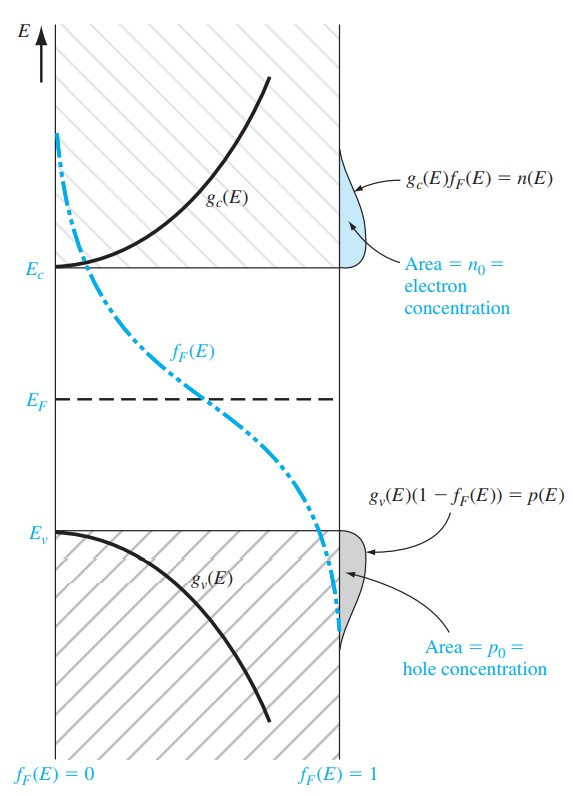
\includegraphics[height=4cm]{Intrinsic.jpg}
                \caption{Intrinsic}
                \label{subfig:Intrinsic.jpg}
            \end{subfigure}
            \begin{subfigure}[b]{0.45\linewidth}
                \centering
                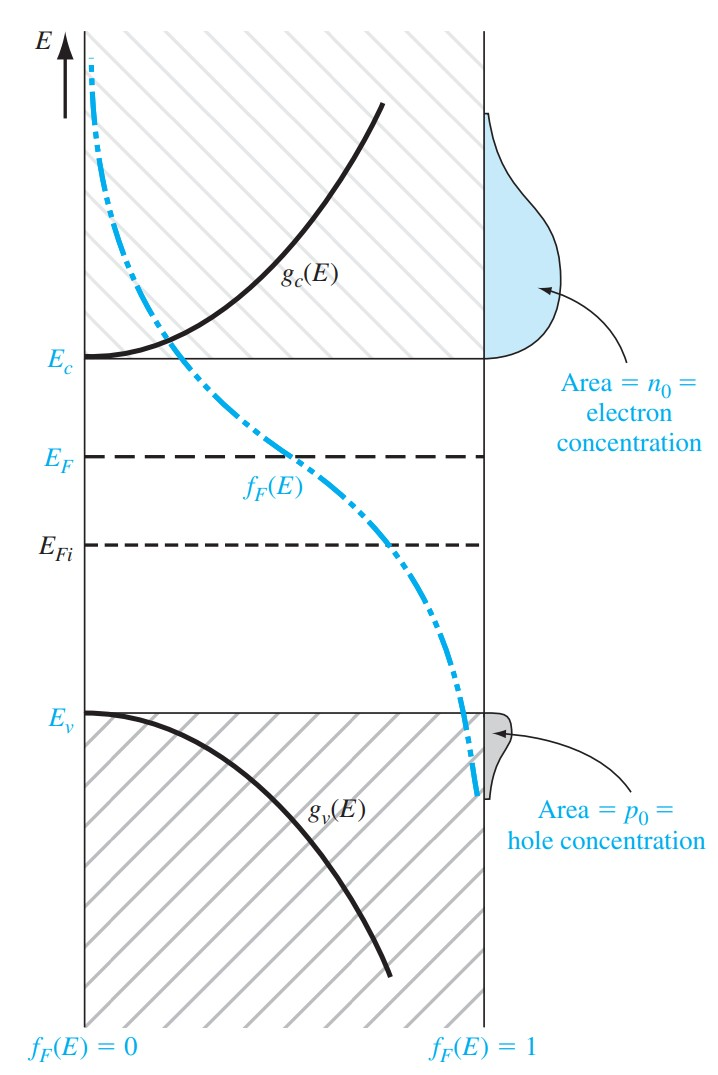
\includegraphics[height=4cm]{Extrinsic-p-type.jpg}
                \caption{n-type semiconductor}
                \label{subfig:Extrinsic-n-type.jpg}
            \end{subfigure}
            \caption{Density of states functions, Fermi-Dirac probability function, and areas representing electron and hole concentrations}
            \label{fig:subcaption-of-dopants}
        \end{figure}
    \end{frame}

    \begin{frame} \frametitle{The Extrinsic Semiconductor}
        \begin{equation*}
            \begin{aligned}
                n_0 &= N_c \exp\left( \frac{E_F - E_c}{kT}  \right) \\
                p_0 &= N_v \exp \left( \frac{E_v - E_F}{kT}  \right)
            \end{aligned}
        \end{equation*}

        \begin{equation*}
            \boxed{n_0p_0 = N_c N_v \exp \left( -\frac{E_g}{kT}  \right) = n_i^2}
        \end{equation*}
    \end{frame}


    \begin{frame} \frametitle{Degenerate Semiconductors}
        \par Impurity concentration increases $\Rightarrow $ distance between impurity atoms decreases $\Rightarrow $ donor electrons start to interact with each other $\Rightarrow $ single discrete donor energy level splits into a band $\Rightarrow $ overlaps with conduction band.
        % \par If the impurity concentration increases, the distance between the impurity atoms decreases and a point will be reached when donor electrons, for example, will begin to interact with each other. When this occurs, the single discrete donor energy will split into a band of energies. As the donor concentration further increases, the band of donor states widens and may overlap the bottom of the conduction band. This overlap occurs when the donor concentration becomes comparable with the effective density of states. When the concentration of electrons in the conduction band exceeds the density of states Nc, the Fermi energy lies within the conduction band.  This type of semiconductor is called a degenerate n-type semiconductor.
        % \par In a similar way, as the acceptor doping concentration increases in a p-type semiconductor, the discrete acceptor energy states will split into a band of energies and may overlap the top of the valence band. The Fermi energy will lie in the valence band when the concentration of holes exceeds the density of states Nv. This type of semiconductor is called a degenerate p-type semiconductor.
    \end{frame}

    \begin{frame} \frametitle{Degenerate Semiconductors}
        \begin{figure}[H]
            \centering
            \begin{subfigure}[b]{0.45\linewidth}
                \centering
                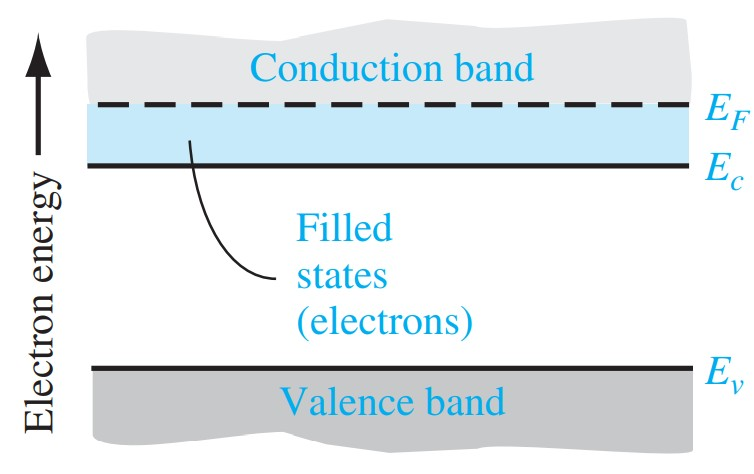
\includegraphics[width=0.9\linewidth]{Degenerate-n.jpg}
                \caption{n-type}
                \label{subfig:Degenerate-n.jpg}
            \end{subfigure}
            \begin{subfigure}[b]{0.45\linewidth}
                \centering
                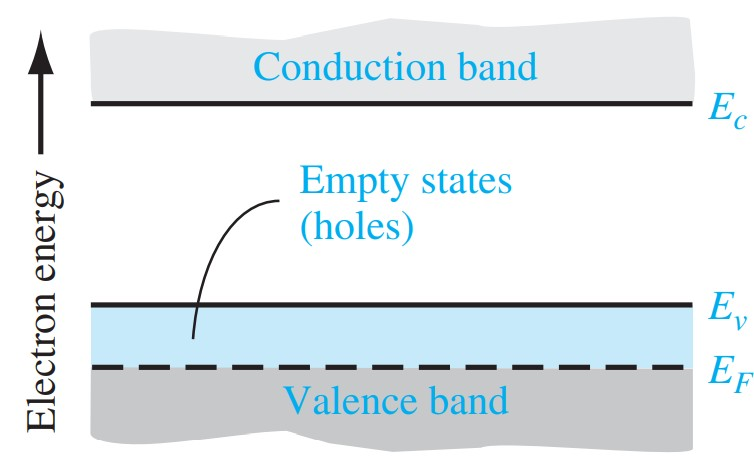
\includegraphics[width=0.9\linewidth]{Degenerate-p.jpg}
                \caption{p-type}
                \label{subfig:Degenerate-p.jpg}
            \end{subfigure}
            \caption{Simplified energy-band diagrams for degenerately doped semiconductors}
            \label{fig:degenerate}
        \end{figure}
        
    \end{frame}

    \begin{frame} \frametitle{Statistics of Donors and Acceptors}
        \begin{equation*}
            f_d(E) = \frac{1}{1 + \frac{1}{2} \exp \left( \frac{E_d - E_F}{kT}  \right)} 
        \end{equation*}
        \begin{equation*}
            n_d = f_d(E) N_d = N_d - N_d^+
        \end{equation*}
        where $N_d^+$ is the concentration of ionized donors.

        \begin{equation*}
            f_a(E) = \frac{1}{1 + \frac{1}{g} \exp\left( \frac{E_F - E_a}{kT}  \right)} 
        \end{equation*}
        $1/g$ is the degeneracy factor, normally taken as $4$ for acceptor level in silicon and gallium arsenide.
        \begin{equation*}
            n_a = f_a(E) N_a = N_a - N_a^+
        \end{equation*}
    \end{frame}


    \begin{frame} \frametitle{Statistics of Donors and Acceptors}
        \par We calculate the relative number of electrons in the donor state compared with the total number of electrons: (assuming $(E_d - E_F) \gg  kT$)
        \begin{equation*}
            \frac{n_d}{n_d + n_0} = \frac{1}{1 + \frac{N_c}{2N_d} \exp\left[ \frac{-(E_c - E_d)}{kT}  \right]} 
        \end{equation*}

        \par \textbf{\textcolor{blue}{Example}:} Determine the fraction of total electrons still in the donor states at $T = 300 K$. Consider phosphorus doping in silicon, for $T = 300 K$, at a concentration of $N_d = 10^{16} cm^{-3}$.
        \par \textbf{\textcolor{blue}{Answer}:} $0.41\%$. Very few electrons remains in the donor states (completely ionized).
    \end{frame}

    % \begin{frame} \frametitle{}
    %     \begin{equation*}
    %         n_0 = \frac{(N_d - N_a)}{2} + \sqrt{\left( \frac{N_d - N_a}{2}  \right)^{2} + n_i^{2} }
    %     \end{equation*}
    % \end{frame}
    \begin{frame} \frametitle{}
        \begin{figure}[H]
            \centering
            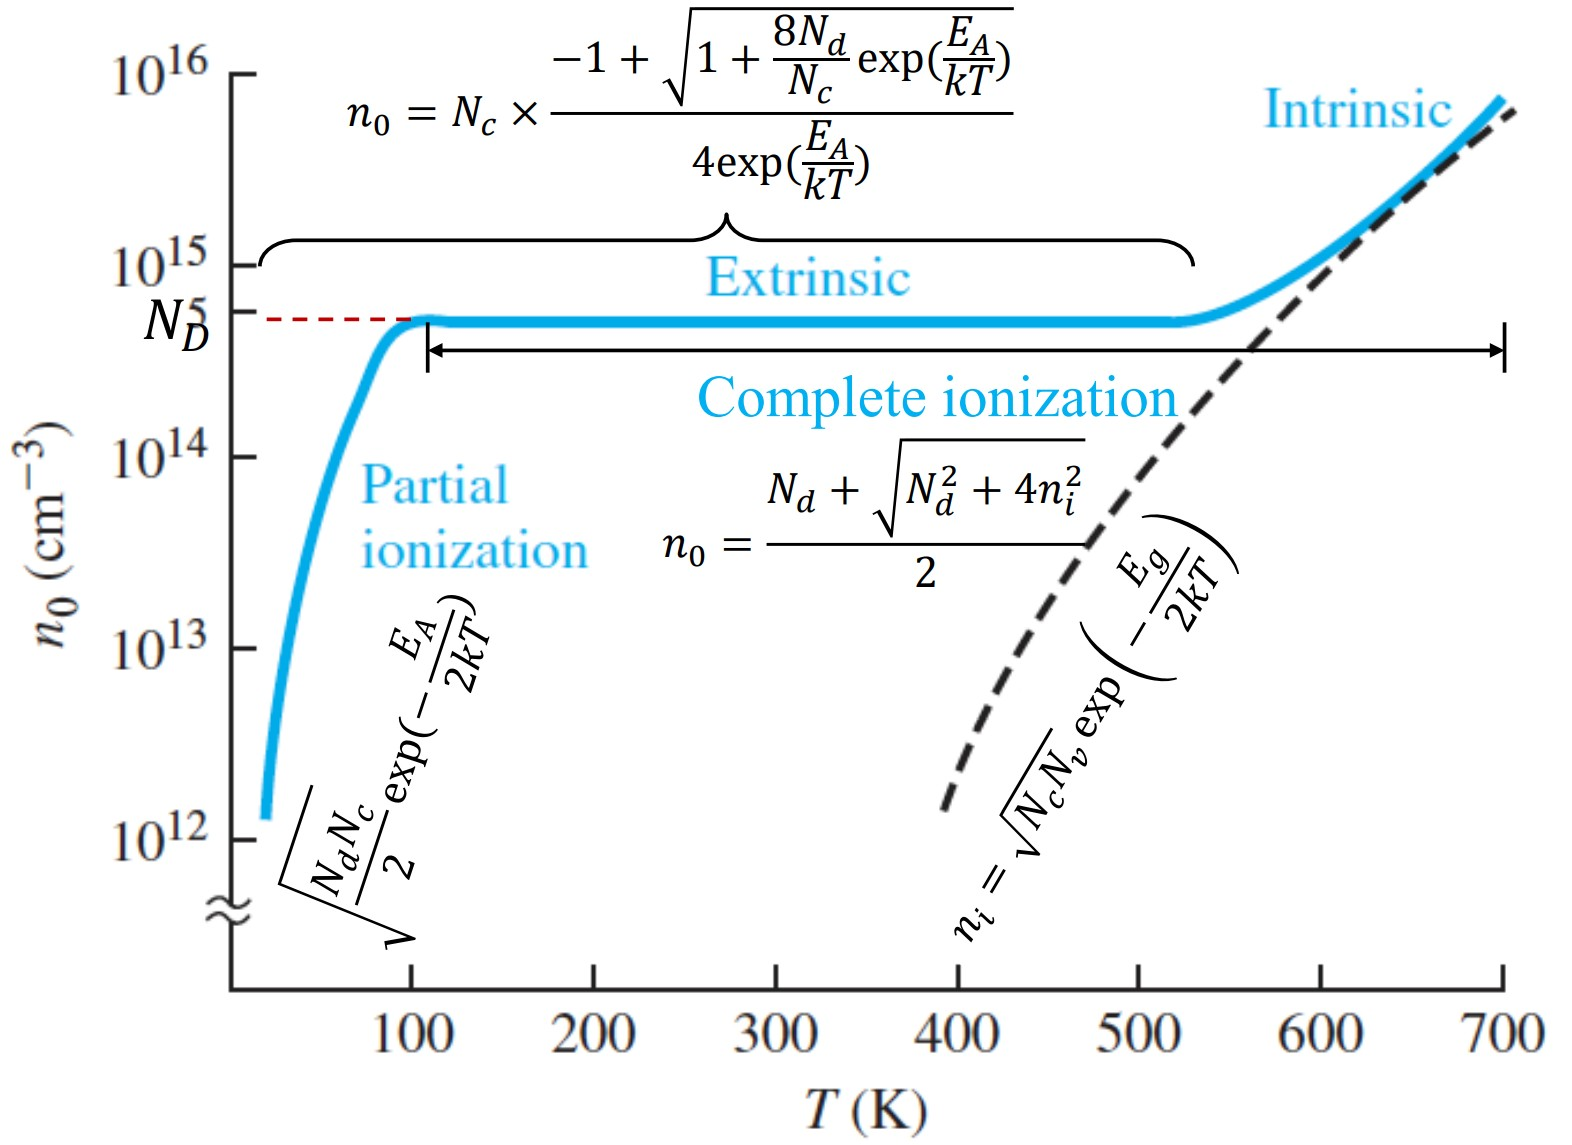
\includegraphics[width=0.95\linewidth]{n0-versus-T.jpg}
            \label{fig:n0-versus-T-0.jpg}
        \end{figure}
    \end{frame}

    \begin{frame} \frametitle{Two Important Equations}
        \begin{equation*}
            \boxed{n_0 = \frac{N_d}{2} + \sqrt{\frac{N_d}{2}^2 + n_i^2 }}
        \end{equation*}
        Charge neutrality:
        \begin{equation*}
            n_0 = p_0 + N_d^+
        \end{equation*}
        Complete ionization:
        \begin{equation*}
            \begin{aligned}
                & n_0 = \frac{n_i^2}{n_0} + N_d \\
                \Rightarrow   \quad & n_0^2 - N_dn_0 - n_i^2 = 0
            \end{aligned}
        \end{equation*}
    \end{frame}
    \begin{frame} \frametitle{Two Important Equations}
        \begin{equation*}
            \boxed{n_0 = N_c \times \frac{-1 + \sqrt{1 + \frac{8N_d}{N_c} \exp\left( \frac{E_A}{kT}  \right)}}{4 \exp \left( \frac{E_A}{kT}  \right)} }
        \end{equation*}
        \begin{equation*}
            n_0 = N_d^+ \quad \text{when $T$ is not high}
        \end{equation*}
        \begin{equation*}
            \begin{aligned}
                n_0 &= \frac{N_d}{1 + 2 \exp\left( \frac{E_F - E_d}{kT}  \right)} \\
                &= \frac{N_d}{1 + 2 \exp \left( \frac{E_c - E_d}{kT}\right)  \exp\left( \frac{E_F - E_c}{kT}  \right)} \\
                &= \frac{N_d}{1 + 2 \exp\left( \frac{E_A}{kT}  \right) \frac{n_0}{N_c} } 
            \end{aligned}
        \end{equation*}
        \begin{equation*}
            \Rightarrow \quad 2 \exp\left( \frac{E_A}{kT}  \right) n_0^2 + N_c n_0 - N_d N_c = 0
        \end{equation*}
    \end{frame}

    \begin{frame} \frametitle{}
        \begin{figure}[H]
            \centering
            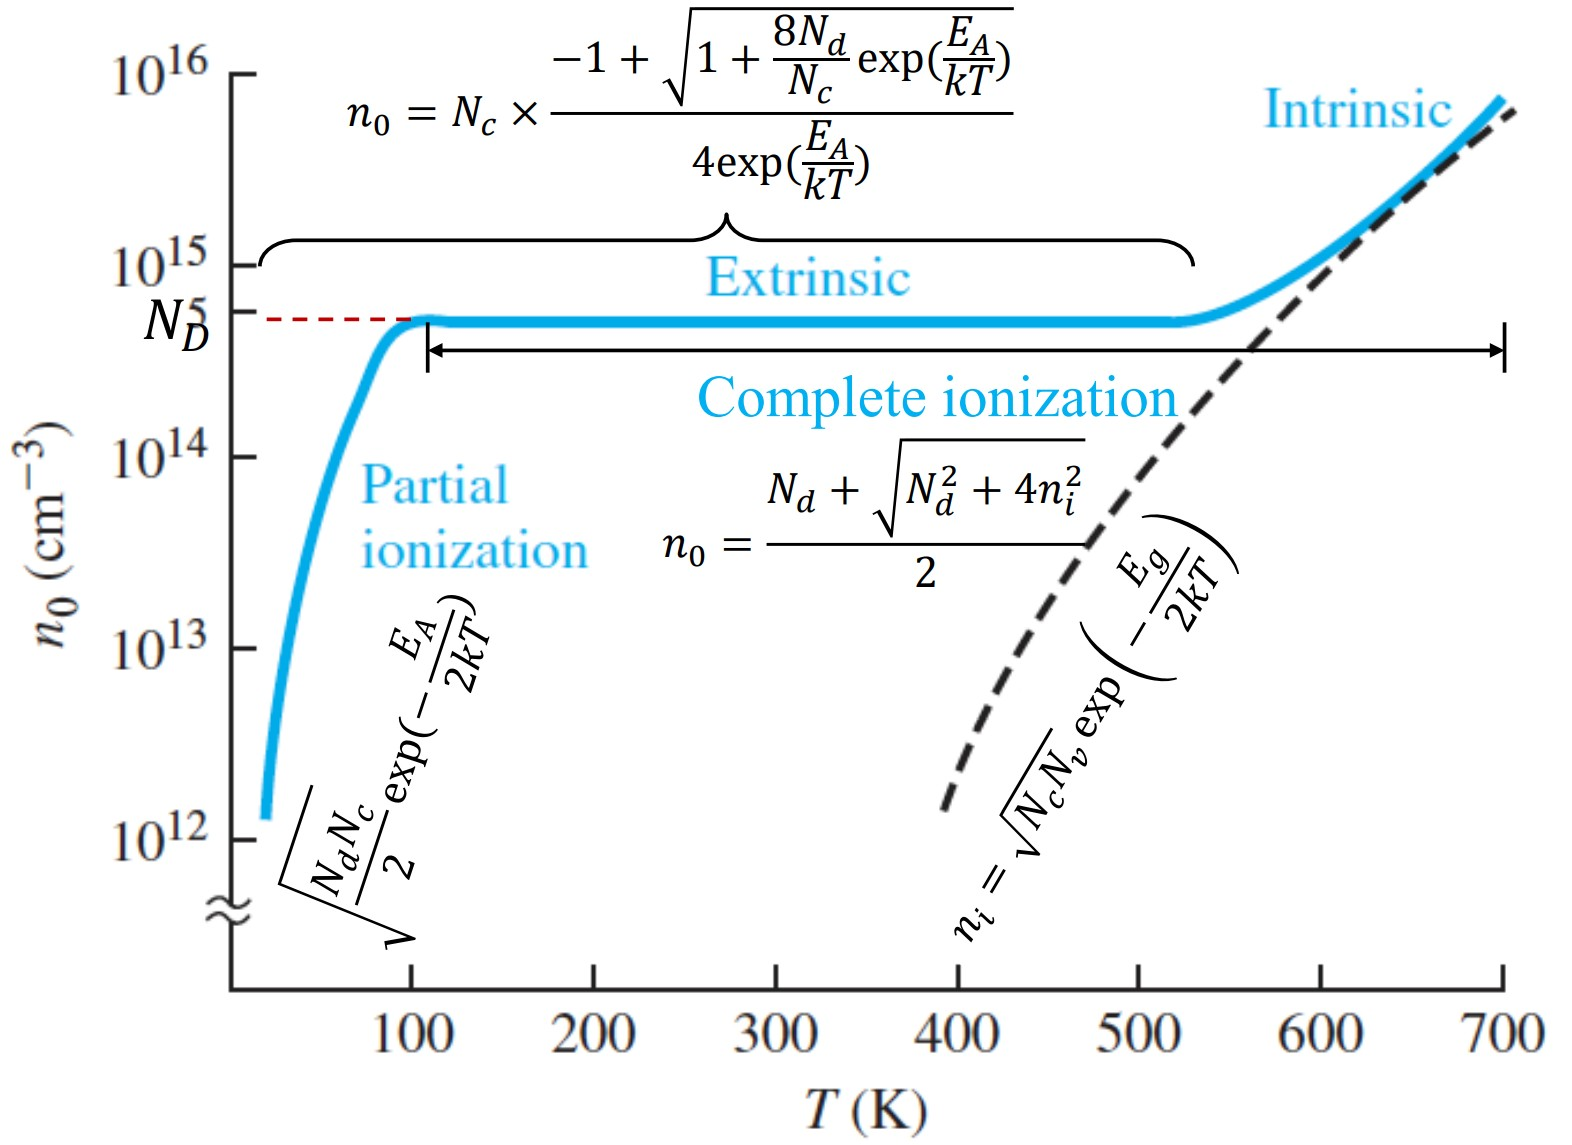
\includegraphics[width=0.95\linewidth]{n0-versus-T.jpg}
            \label{fig:n0-versus-T.jpg}
        \end{figure}
    \end{frame}

    \begin{frame} \frametitle{Fermi Level Position}
        \begin{equation*}
            \begin{aligned}
                E_F &= E_c + kT \ln \left( \frac{\sqrt{1 + \frac{8 N_d}{N_c} \exp\left( \frac{E_A}{kT}  \right)} - 1}{4 \exp\left( \frac{E_A}{kT}  \right)}  \right) \\
                &= \left\{
                    \begin{aligned}
                        \frac{E_c + E_D}{2} +\frac{kT}{2} \ln \frac{N_d}{2N_c}, &\quad  T \text{ small} \\
                        E_c - kT \ln \frac{N_c}{N_d}, &\quad  T \text{ big}
                    \end{aligned}
                \right.
            \end{aligned}
        \end{equation*}
        \begin{figure}[H]
            \centering
            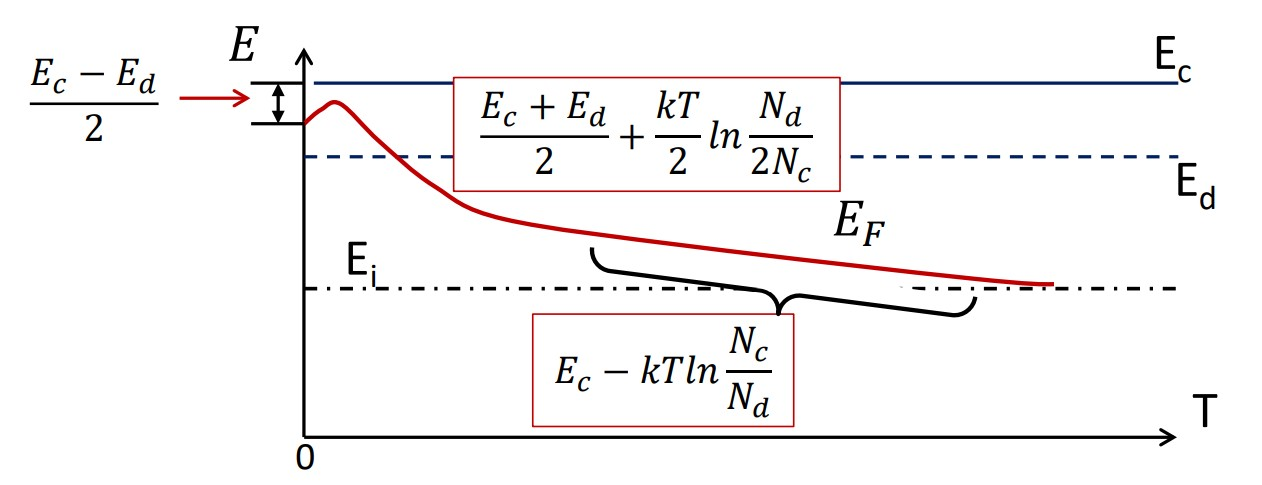
\includegraphics[width=0.8\linewidth]{Fermi-level-position.jpg}
            \label{fig:Fermi-level-position.jpg}
        \end{figure}
    \end{frame}


\section{Chapter 5-I Carrier Transport Phenomena}
\subsection{Drift}
    \begin{frame} \frametitle{Drift}
        \begin{figure}[H]
            \centering
            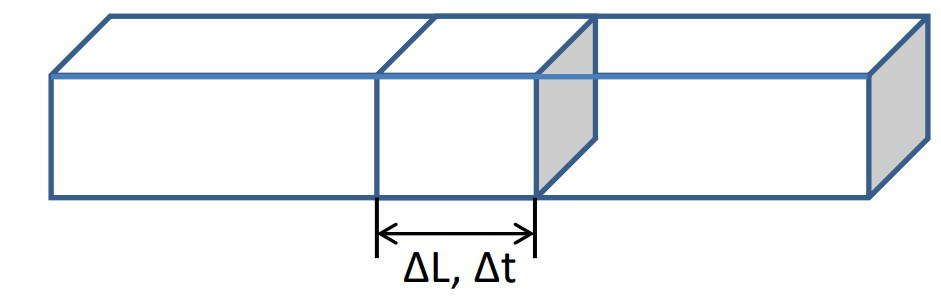
\includegraphics[width=0.6\linewidth]{Drift.jpg}
            \caption{for p type semiconductor ($p_0 \gg n_0$)}
            \label{fig:Drift.jpg}
        \end{figure}
        
        \begin{equation*}
            I_{drf} = \frac{\Delta Q}{\Delta t} = \frac{qp_0 A_c \Delta L}{\Delta t} = qp_0 A_c v_d 
        \end{equation*}

        How to derive $v_d$?

        \begin{equation*}
            v = \frac{qEt}{m^*_{cp}} ,
        \end{equation*}
        \par where $\tau_{cp}$ - the mean time between collisions
        \begin{equation*}
            v_d \approx \left( \frac{q \tau_{cp}}{m^*_{cp}}  \right) E = \mu_p E
        \end{equation*}
    \end{frame}

    \begin{frame} \frametitle{Drift}
        \begin{equation*}
            \boxed{J_{drf} = q (p_0 \mu_p + n_0 \mu_n) E}
        \end{equation*}
        \begin{equation*}
            \begin{aligned}
                & \rho = \frac{1}{\sigma} = \frac{1}{q(\mu_n n + \mu_p p)} \\
                & \rho:  \text{resistivity} \\
                & \sigma:  \text{conductivity}
            \end{aligned}
        \end{equation*}
        \begin{figure}[H]
            \centering
            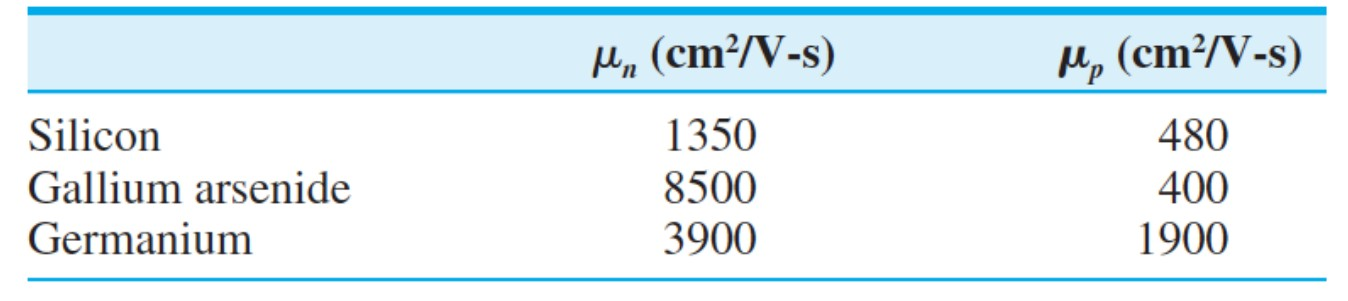
\includegraphics[width=0.9\linewidth]{Typical-mobility.jpg}
            \caption{Typical mobility values at $T = 300K$ and low doping concentrations}
            \label{fig:Typical-mobility.jpg}
        \end{figure}
    \end{frame}


    \begin{frame} \frametitle{Example}
        \par A bar of p-type silicon at $300K$ in the figure below has a cross-sectional area $A = 10^{-6} cm^2$ and a length $L = 1.2 \times 10^{-3} cm$. For an applied voltage of $5V$, a current of $2mA$ is required. What is the required (a) resistance, (b) resistivity, and (c) impurity doping concentration? (d) What is the resulting hole mobility? ($p = 7 \times 10^{15} cm^{-3}$)
        \begin{figure}[H]
            \begin{flushleft}
                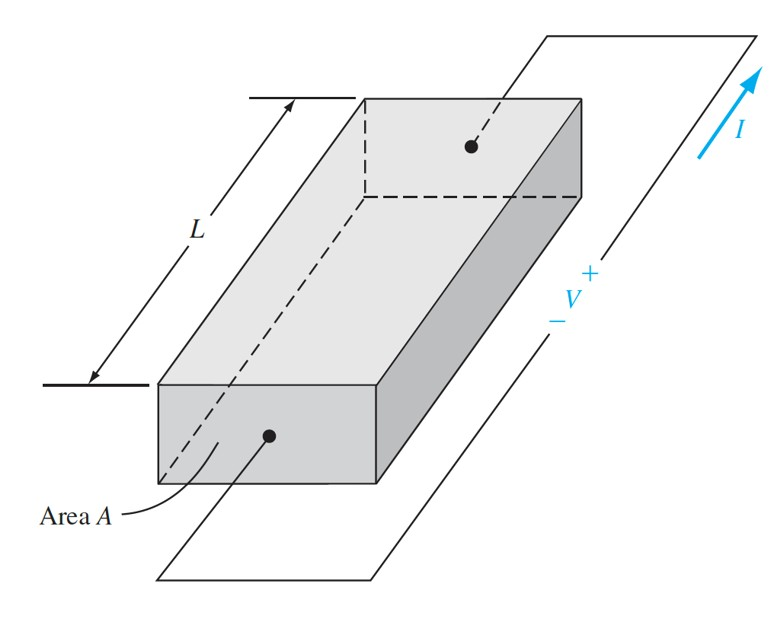
\includegraphics[width=0.6\linewidth]{Example.jpg}
            \end{flushleft}
            \label{fig:Example.jpg}
        \end{figure}
        
    \end{frame}

    \begin{frame} \frametitle{Mobility Effect - Scattering}
        \begin{itemize}
            \item \textit{Lattice scattering / phonon scattering} \\
                Lattice scatterings shorten $\tau_{cp}$ $\implies \mu_L \propto T^{-3/2}$
            \item \textit{Ionized impurity scattering} \\
                Impurity scatterings shorten $\tau_{cp}$ $\implies \mu_I \propto \frac{T^{3/2}}{N_d^+ + N_a^-} $
        \end{itemize}

        \begin{equation*}
            \frac{1}{\mu} = \frac{1}{\mu_L} + \frac{1}{\mu_I} 
        \end{equation*}

        \begin{figure}[H]
            \centering
            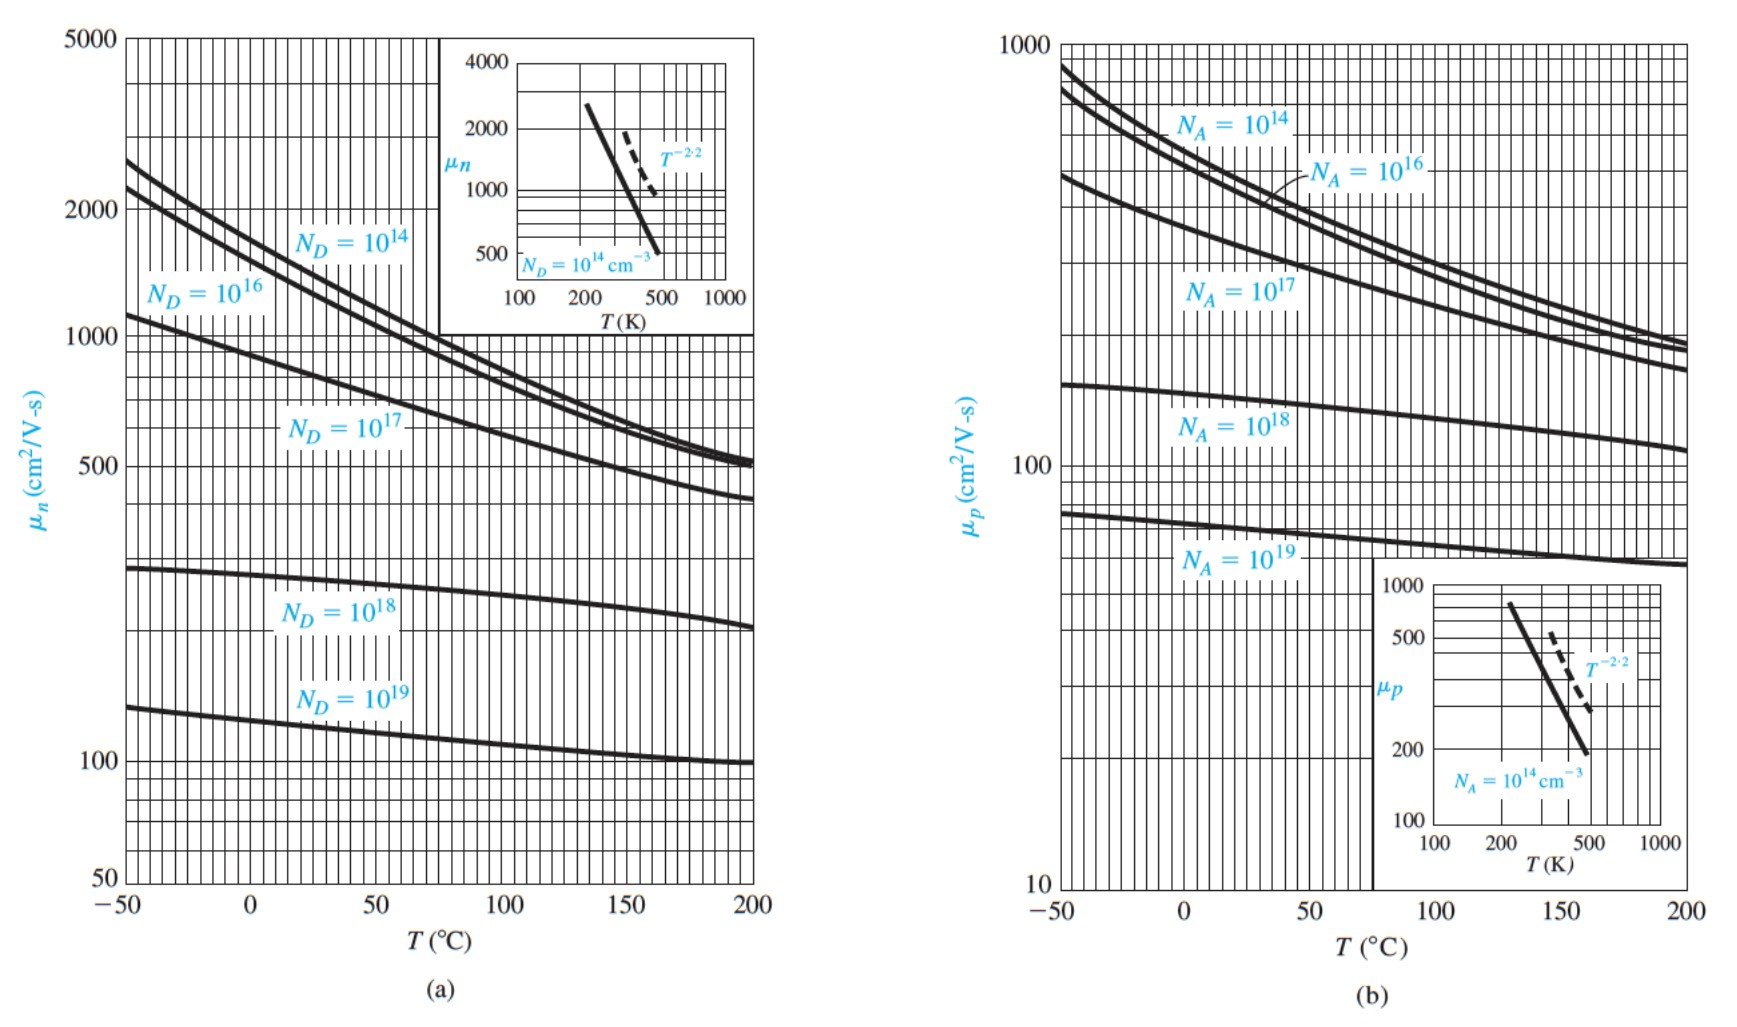
\includegraphics[width=0.7\linewidth]{Mobility-effect.jpg}
            \label{fig:Mobility-effect.jpg}
        \end{figure}
    \end{frame}


    \begin{frame} \frametitle{Velocity Saturation}
        \begin{figure}[H]
            \centering
            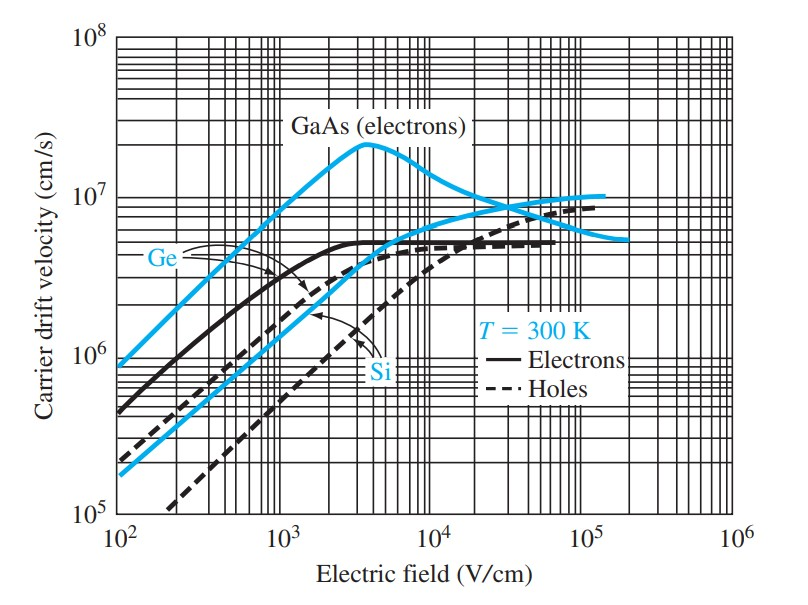
\includegraphics[width=0.5\linewidth]{Velocity-saturation.jpg}
            \label{fig:Velocity-saturation.jpg}
        \end{figure}
        \begin{equation*}
            \begin{aligned}
                v_n &= \frac{v_s}{\left[ 1 + \left( \frac{E_{on}}{E}  \right)^2 \right]^{1/2}} \\
                v_p &= \frac{v_s}{\left[ 1 + \left( \frac{E_{op}}{E}  \right)^2 \right]^{1/2}} 
            \end{aligned}
        \end{equation*}
        In silicon at $T = 300K$, $v_s = 10^7 cm /s$, $E_{on} = 7 \times 10^3 V /cm$, $E_{op} = 2 \times 10^4 V / cm$.
        
    \end{frame}


\subsection{Diffusion}
    \begin{frame} \frametitle{Diffusion}
        \begin{figure}[H]
            \centering
            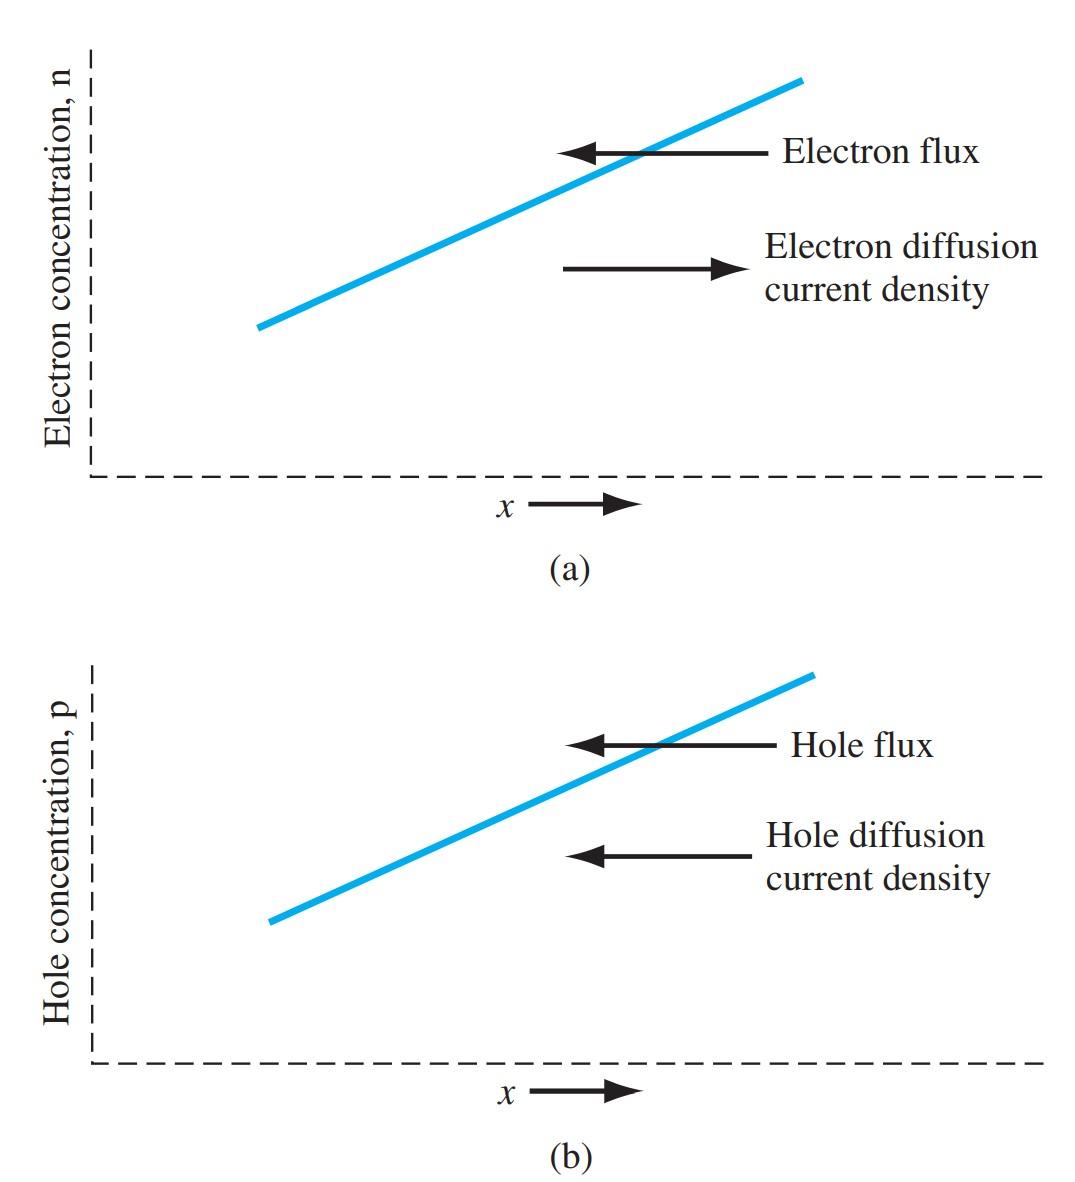
\includegraphics[width=0.4\linewidth]{Diffusion.jpg}
            \caption{(a) Diffusion of electrons due to a density gradient. (b) Diffusion of holes due to a density gradient.}
            \label{fig:Diffusion.jpg}
        \end{figure}
        \begin{equation*}
            \begin{aligned}
                J_{nx|dif} &= eD_n \frac{\d n}{\d x} \\
                J_{px|dif} &= -e D_p \frac{\d p}{\d x} 
            \end{aligned}
        \end{equation*}
    \end{frame}

    \begin{frame} 
        \begin{center}
            \Large\textcolor{blue}{End}
        \end{center}
    \end{frame}

\end{document} 